%%%%%%%%%%%%%%%%%%%%%%%%%%%%%%%%%%

\section{ANOVAによる平均の比較}

%%%%%%%%%%%%%%%%%%%%%%%%%%%%%%%%%%%

\subsection{ウルフ川のアルドリン}

%%%%%%%%%%%%%%%%%%%%%%%%%%%%%%%%%%%

\begin{frame}
\frametitle{}

\begin{center}
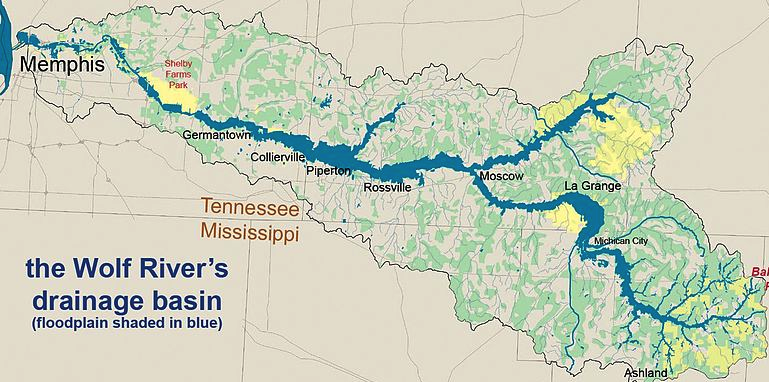
\includegraphics[width=0.5\textwidth]{7-5_anova/figures/aldrin/wolf}
\end{center}

{\small
\begin{itemize}

\item テネシー州のウルフ川は、殺虫剤産業がクロルダン（農薬）、アルドリン、ディエルドリン（いずれも殺虫剤）などの廃棄物を捨てていたかつての廃棄場跡地のそばを流れている。

\item これらの高毒性有機化合物は、様々な種類のがんや先天性異常を引き起こす可能性がある。

\item これらの物質が川に存在するかどうかを検定する標準的な方法は、深さの10分の6の深さで採取することである。

\item しかし、これらの化合物は水よりも密度が高く、分子が堆積粒子に付着する傾向があるため、中深度よりも底部付近でより高い濃度で見られる可能性が高い。

\end{itemize}
}

\end{frame}

%%%%%%%%%%%%%%%%%%%%%%%%%%%%%%%%%%%

\begin{frame}
\frametitle{データ}

3つの深さレベルでのアルドリン濃度（ナノグラム/リットル）。\\

\begin{center}
\begin{tabular}{r | c | c}
\hline
 	& アルドリン 					& 深さ \\
\hline
1 	& \textcolor{darkGray}{3.80} 	& \textcolor{darkGray}{底部}  \\
2 	& \textcolor{darkGray}{4.80} 	& \textcolor{darkGray}{底部}  \\
...	&						& \\
10	& \textcolor{darkGray}{8.80} 	& \textcolor{darkGray}{底部} \\
11	& \textcolor{blue}{3.20} 		& \textcolor{blue}{中深度}  \\
12	& \textcolor{blue}{3.80} 		& \textcolor{blue}{中深度} \\
...	&						& \\
20 	& \textcolor{blue}{6.60} 		& \textcolor{blue}{中深度} \\
21	& \textcolor{oiB}{3.10} 		& \textcolor{oiB}{表面} \\
22	& \textcolor{oiB}{3.60} 		& \textcolor{oiB}{表面} \\
...	&						& \\
30 	& \textcolor{oiB}{5.20} 		& \textcolor{oiB}{表面} \\
\hline
\end{tabular}
\end{center}

\end{frame}

%%%%%%%%%%%%%%%%%%%%%%%%%%%%%%%%%%%

\begin{frame}
\frametitle{探索的分析}

3つの深さレベルでのアルドリン濃度（ナノグラム/リットル）。\\

\begin{center}
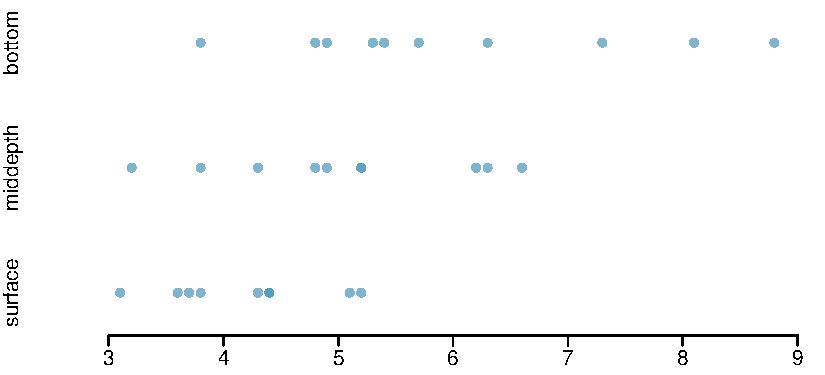
\includegraphics[width=0.75\textwidth]{7-5_anova/figures/aldrin/dotplot}
\end{center}

\begin{center}
\begin{tabular}{l | c c c}
		& n	& 平均	& 標準偏差	\\
\hline
底部	& 10	& 6.04	& 1.58 \\
中深度	& 10	& 5.05	& 1.10 \\
表面	& 10	& 4.20	& 0.66 \\
\hline
全体	& 30	& 5.10	& 1.37
\end{tabular}
\end{center}

\end{frame}

%%%%%%%%%%%%%%%%%%%%%%%%%%%%%%%%%%%

\begin{frame}
\frametitle{研究の問い}

\dq{3つの深さレベル間でアルドリン濃度の平均に差があるか？}

\vspace{0.5cm}

\begin{itemize}

\item 2グループの平均を比較するには$Z$または$T$統計量を使う。

\item 3グループ以上の平均を比較するには、\hl{ANOVA（分散分析）}という新しい検定と\hl{$F$}という新しい統計量を使う。

\end{itemize}

\end{frame}

%%%%%%%%%%%%%%%%%%%%%%%%%%%%%%%%%%%

\begin{frame}
\frametitle{ANOVA（分散分析）}

ANOVAは、目的変数の平均がカテゴリ変数の異なるレベルで異なるかどうかを評価するために使われる。

\begin{itemize}
\item[] \mathhl{H_0:} すべてのカテゴリで目的変数の平均は同じである。
\[\mu_1 = \mu_2 = \cdots = \mu_k, \]
ここで$\mu_i$はカテゴリ$i$の観測値の目的変数の平均を表す。
\item[]
\item[] \mathhl{H_A:} 少なくとも1つの平均が他と異なる。
\end{itemize}

\end{frame}

%%%%%%%%%%%%%%%%%%%%%%%%%%%%%%%%%%%

\begin{frame}
\frametitle{条件の確認}

\begin{enumerate}

\item 観測値はグループ内およびグループ間で独立でなければならない。

\begin{itemize}
\item データが母集団の10\%未満の単純無作為標本であれば、この条件は満たされる。
\item データが独立かどうかを注意深く考える（例えば、対になっていないか）。
\item 常に重要だが、確認が難しい場合もある。
\end{itemize}

\item 各グループ内の観測値はほぼ正規分布に従う必要がある。

\begin{itemize}
\item 標本サイズが小さい場合に特に重要である。
\end{itemize}

\dq{正規性はどのように確認するか？}

\item グループ間の変動性はほぼ等しい必要がある。

\begin{itemize}
\item グループ間で標本サイズが異なる場合に特に重要である。
\end{itemize}

\dq{この条件はどのように確認できるか？}

\end{enumerate}

\end{frame}

%%%%%%%%%%%%%%%%%%%%%%%%%%%%%%%%%%%

\begin{frame}
\frametitle{$z$/$t$検定 vs. ANOVA - 目的}

\twocol{0.5}{0.5}
{
\[ \hl{$z$/$t$検定} \]
\hl{2つ}のグループの平均を比較し、観察された差がサンプリング変動によって合理的に説明できないほど離れているかどうかを見る。
\[ H_0: \mu_1 = \mu_2 \]
}
{
\[ \hl{ANOVA} \]
\hl{2つ以上}のグループの平均を比較し、観察された差がすべてサンプリング変動によって合理的に説明できないほど離れているかどうかを見る。
\[ H_0: \mu_1 = \mu_2 = \cdots = \mu_k \]
}

\end{frame}

%%%%%%%%%%%%%%%%%%%%%%%%%%%%%%%%%%%

\begin{frame}
\frametitle{$z$/$t$検定 vs. ANOVA - 方法}

\twocol{0.5}{0.5}
{
\[ \hl{$z$/$t$検定} \]
検定統計量（比）を計算する。
\[ z / t = \frac{(\bar{x}_1 - \bar{x}_2) - (\mu_1 - \mu_2)}{SE(\bar{x}_1 - \bar{x}_2)} \]
}
{
\[ \hl{ANOVA} \]
検定統計量（比）を計算する。
\[ F = \frac{\text{群間変動}}{\text{群内変動}} \]
}

\vspace{1cm}

\begin{itemize}

\item 大きな検定統計量は小さなp値をもたらす。

\item p値が十分小さければ$H_0$は棄却され、母集団平均は等しくないと結論付ける。

\end{itemize}

\end{frame}

%%%%%%%%%%%%%%%%%%%%%%%%%%%%%%%%%%%

\begin{frame}
\frametitle{$z$/$t$検定 vs. ANOVA}

\begin{itemize}

\item グループが2つだけの場合、検定統計量の分母にプールされた分散を使えば$t$検定とANOVAは等価となる。

\item グループが3つ以上の場合、ANOVAは標本平均を全体の\hl{総平均}と比較する。

\end{itemize}

\end{frame}

%%%%%%%%%%%%%%%%%%%%%%%%%%%%%%%%%%%

\begin{frame}
\frametitle{仮説}

\pq{3つの深さレベル間でアルドリン濃度の平均に差があるかを検定するための正しい仮説はどれか？}

\begin{enumerate}[(a)]
\item $H_0: \mu_B = \mu_M = \mu_S$ \\
$H_A: \mu_B \ne \mu_M \ne \mu_S$ \\
\item $H_0: \mu_B \ne \mu_ M \ne \mu_S$ \\
$H_A: \mu_B = \mu_M = \mu_S$ \\
\solnMult{$H_0: \mu_B = \mu_M = \mu_S$ \\
$H_A:$ 少なくとも1つの平均が他と異なる。}
\item $H_0: \mu_B = \mu_M = \mu_S = 0$ \\
$H_A:$ 少なくとも1つの平均が他と異なる。
\item $H_0: \mu_B = \mu_M = \mu_S$ \\
$H_A: \mu_B > \mu_M > \mu_S$ \\
\end{enumerate}

\end{frame}

%%%%%%%%%%%%%%%%%%%%%%%%%%%%%%%%%%%

\subsection{ANOVAとF検定}

%%%%%%%%%%%%%%%%%%%%%%%%%%%%%%%%%%%

\begin{frame}
\frametitle{検定統計量}

\dq{グループ内の変動は大きく見えるか？グループ間はどうか？}

\[ F = \frac{\text{群間変動}}{\text{群内変動}}  \]

\begin{center}
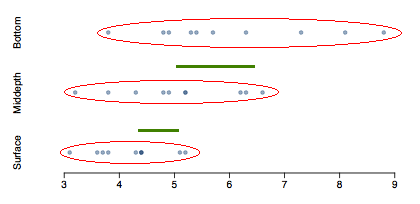
\includegraphics[width=0.75\textwidth]{7-5_anova/figures/aldrin/dotplot_var}
\end{center}

\end{frame}

%%%%%%%%%%%%%%%%%%%%%%%%%%%%%%%%%%%

\begin{frame}
\frametitle{$F$分布とp値}

\[ F =  \frac{\text{群間変動}}{\text{群内変動}} \]

\vspace{-1cm}

\begin{center}
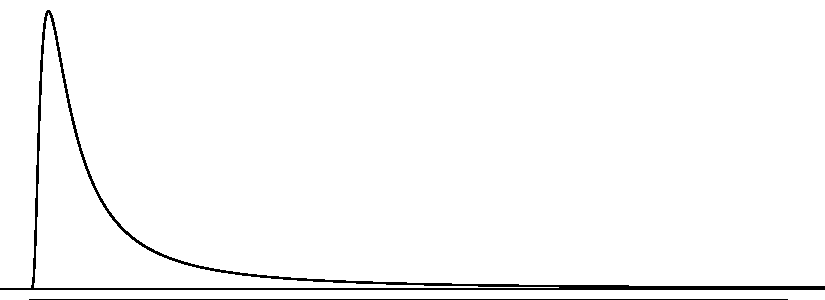
\includegraphics[width=0.75\textwidth]{7-5_anova/figures/fdist/fdist}
\end{center}

\begin{itemize}

\item $H_0$を棄却するためには小さなp値が必要であり、そのためには大きな$F$統計量が必要である。

\item 大きな$F$統計量を得るためには、標本平均間の変動がグループ内の変動よりも大きい必要がある。

\end{itemize}

\end{frame}

%%%%%%%%%%%%%%%%%%%%%%%%%%%%%%%%%%%

\subsection{ANOVA出力の解説}

%%%%%%%%%%%%%%%%%%%%%%%%%%%%%%%%%%%

\begin{frame}
\frametitle{}

\vspace{-0.5cm}

{\footnotesize
\begin{center}
\begin{tabular}{ll >{\columncolor[gray]{.6}[.5\tabcolsep]}rrrrr}
\hline
 			& 			& Df 	& Sum Sq	& Mean Sq 	& F value 	& Pr($>$F) \\
\hline
(\hl{G}roup) 	& depth 		& 2 	& 16.96 	& 8.48 		& 6.13 	& 0.0063 \\
(\hl{E}rror) 	& Residuals 	& 27 	& 37.33 	& 1.38 		&  		&  \\
\hline
	 		& \hl{T}otal	& 29	& 54.29 \\
\end{tabular}
\end{center}
}

\formula{ANOVAに関連する自由度}
{
\begin{itemize}
\item グループ：$df_G = k - 1$，ここで$k$はグループ数
\item 全体：$df_T = n - 1$，ここで$n$は総標本サイズ
\item 誤差：$df_E = df_T - df_G$
\end{itemize}
}

\begin{itemize}

\item $df_G = k - 1 = 3 - 1 = 2$ \\

\item $df_T = n - 1 = 30 - 1 = 29$

\item $df_E = 29 - 2 = 27$ \\

\end{itemize}

\end{frame}

%%%%%%%%%%%%%%%%%%%%%%%%%%%%%%%%%%%

\begin{frame}
\frametitle{}

\vspace{-0.25cm}

{\footnotesize
\begin{center}
\begin{tabular}{ll r>{\columncolor[gray]{.6}[.5\tabcolsep]}rrrr}
\hline
 			& 			& Df 	& Sum Sq	& Mean Sq 	& F value 	& Pr($>$F) \\
\hline
(\hl{G}roup) 	& depth 		& 2 	& \orange{16.96} 	& 8.48 		& 6.13 	& 0.0063 \\
(\hl{E}rror) 	& Residuals 	& 27 	& 37.33 	& 1.38 		&  		&  \\
\hline
	 		& \hl{T}otal	& 29	& 54.29 \\
\end{tabular}
\end{center}
}

\formula{グループ間の平方和，SSG}
{
グループ間の変動を測る
\vspace{-0.25cm}
\[ SSG = \sum_{i = 1}^{k} n_i (\bar{x}_i - \bar{x})^2 \]
ここで$n_i$は各グループサイズ，$\bar{x}_i$は各グループの平均，$\bar{x}$は全体（総）平均。
}

\vspace{-0.5cm}

\twocol{0.4}{0.5}
{
{\small
\begin{center}
\begin{tabular}{l | c c }
		& n	& 平均		\\
\hline
底部	& 10	& 6.04	 \\
中深度	& 10	& 5.05	 \\
表面	& 10	& 4.2	 \\
\hline
全体	& 30	& 5.1
\end{tabular}
\end{center}
}
}
{
\begin{eqnarray*}
SSG &=& \pr{ 10 \times (6.04 - 5.1)^2 } \\
&+& \pr{ 10 \times (5.05 - 5.1)^2 } \\
&+& \pr{ 10 \times (4.2 - 5.1)^2 } \\
&=& 16.96 \\
\end{eqnarray*}
}

\end{frame}

%%%%%%%%%%%%%%%%%%%%%%%%%%%%%%%%%%%

\begin{frame}
\frametitle{}

\vspace{-0.25cm}

{\footnotesize
\begin{center}
\begin{tabular}{ll r>{\columncolor[gray]{.6}[.5\tabcolsep]}rrrr}
\hline
 			& 			& Df 	& Sum Sq	& Mean Sq 	& F value 	& Pr($>$F) \\
\hline
(\hl{G}roup) 	& depth 		& 2 	& 16.96	& 8.48 		& 6.13 	& 0.0063 \\
(\hl{E}rror) 	& Residuals 	& 27 	& 37.33 	& 1.38 		&  		&  \\
\hline
	 		& \hl{T}otal	& 29	& \orange{54.29} \\
\end{tabular}
\end{center}
}

\formula{全体の平方和，SST}
{
全体の変動を測る
\vspace{-0.25cm}
\[ SST = \sum_{i = 1}^{n} (x_i - \bar{x})^2 \]
ここで$x_i$はデータセットの各観測値を表す。
}

\vspace{-0.75cm}

{\small
\begin{eqnarray*}
SST &=& (3.8 - 5.1)^2 + (4.8 - 5.1)^2 + (4.9 - 5.1)^2 + \cdots + (5.2 - 5.1)^2 \\
&=& (-1.3)^2 + (-0.3)^2 + (-0.2)^2 + \cdots + (0.1)^2 \\
&=& 1.69 + 0.09 + 0.04 + \cdots + 0.01 \\
&=& 54.29
\end{eqnarray*}
}

\end{frame}

%%%%%%%%%%%%%%%%%%%%%%%%%%%%%%%%%%%

\begin{frame}
\frametitle{}

\vspace{-0.25cm}

{\footnotesize
\begin{center}
\begin{tabular}{ll r>{\columncolor[gray]{.6}[.5\tabcolsep]}rrrr}
\hline
 			& 			& Df 	& Sum Sq	& Mean Sq 	& F value 	& Pr($>$F) \\
\hline
(\hl{G}roup) 	& depth 		& 2 	& 16.96	& 8.48 		& 6.13 	& 0.0063 \\
(\hl{E}rror) 	& Residuals 	& 27 	& \orange{37.33} 	& 1.38 		&  		&  \\
\hline
	 		& \hl{T}otal	& 29	& 54.29 \\
\end{tabular}
\end{center}
}

\formula{誤差の平方和，SSE}
{
グループ内の変動を測る：
\[ SSE = SST - SSG \]
}

\[ SSE =  54.29 - 16.96 =  37.33 \]

\end{frame}

%%%%%%%%%%%%%%%%%%%%%%%%%%%%%%%%%%%

\begin{frame}
\frametitle{}

\vspace{-0.25cm}

{\footnotesize
\begin{center}
\begin{tabular}{ll rr>{\columncolor[gray]{.6}[.5\tabcolsep]}rrr}
\hline
 			& 			& Df 	& Sum Sq	& Mean Sq 	& F value 	& Pr($>$F) \\
\hline
(\hl{G}roup) 	& depth 		& 2 	& 16.96	& \orange{8.48} 		& 6.13 	& 0.0063 \\
(\hl{E}rror) 	& Residuals 	& 27 	& 37.33 	& \orange{1.38} 		&  		&  \\
\hline
	 		& \hl{T}otal	& 29	& 54.29 \\
\end{tabular}
\end{center}
}

\formula{平均二乗誤差}
{
平均二乗誤差は平方和を自由度で割って計算される。
}

\begin{eqnarray*}
MSG &=& 16.96 / 2 = 8.48 \\
MSE &=& 37.33 / 27 = 1.38
\end{eqnarray*}

\end{frame}

%%%%%%%%%%%%%%%%%%%%%%%%%%%%%%%%%%%

\begin{frame}
\frametitle{}

\vspace{-0.25cm}

{\footnotesize
\begin{center}
\begin{tabular}{ll rrr>{\columncolor[gray]{.6}[.5\tabcolsep]}rr}
\hline
 			& 			& Df 	& Sum Sq	& Mean Sq 	& F value 	& Pr($>$F) \\
\hline
(\hl{G}roup) 	& depth 		& 2 	& 16.96	& 8.48 		& \orange{6.14} 	& 0.0063 \\
(\hl{E}rror) 	& Residuals 	& 27 	& 37.33 	& 1.38 		&  		&  \\
\hline
	 		& \hl{T}otal	& 29	& 54.29 \\
\end{tabular}
\end{center}
}

\formula{検定統計量，F値}
{
先に述べたように、F統計量はグループ間変動とグループ内変動の比である。
\[ F = \frac{MSG}{MSE} \]
}

\[ F = \frac{8.48}{1.38} = 6.14 \]

\end{frame}

%%%%%%%%%%%%%%%%%%%%%%%%%%%%%%%%%%%

\begin{frame}
\frametitle{}

\vspace{-0.25cm}

{\footnotesize
\begin{center}
\begin{tabular}{ll rrr>{\columncolor[gray]{.6}[.5\tabcolsep]}rr}
\hline
 			& 			& Df 	& Sum Sq	& Mean Sq 	& F value 	& Pr($>$F) \\
\hline
(\hl{G}roup) 	& depth 		& 2 	& 16.96	& 8.48 		& \orange{6.14} 	& 0.0063 \\
(\hl{E}rror) 	& Residuals 	& 27 	& 37.33 	& 1.38 		&  		&  \\
\hline
	 		& \hl{T}otal	& 29	& 54.29 \\
\end{tabular}
\end{center}
}

\formula{p値}
{
p値は、すべてのグループの平均が等しいとした場合に、「グループ間」変動と「グループ内」変動の比が観察された値以上となる確率である。自由度$df_G$と$df_E$のF曲線の下で観察されたF統計量より右側の面積として計算される。
}

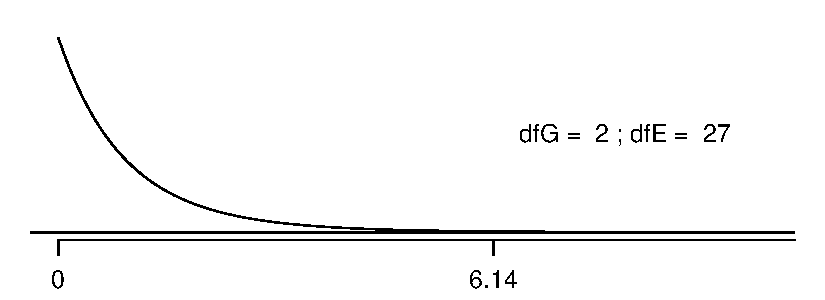
\includegraphics[width=0.9\textwidth]{7-5_anova/figures/aldrin/f}

\end{frame}

%%%%%%%%%%%%%%%%%%%%%%%%%%%%%%%%%%%

\begin{frame}
\frametitle{結論 - 文脈の中で}

\pq{仮説検定の結論は何か？}

$\:$ \\

データは、アルドリンの平均濃度が

\begin{enumerate}[(a)]

\item すべてのグループで異なることの説得力ある証拠を提供している。

\item 表面では他のレベルよりも低いことの説得力ある証拠を提供している。

\solnMult{少なくとも1つのグループで異なることの説得力ある証拠を提供している。}

\item すべてのグループで同じであることの説得力ある証拠を提供している。

\end{enumerate}

\end{frame}

%%%%%%%%%%%%%%%%%%%%%%%%%%%%%%%%%%%

\begin{frame}
\frametitle{結論}

\begin{itemize}

\item p値が小さい（$\alpha$未満）場合、$H_0$を棄却する。データは少なくとも1つの平均が他と異なることの説得力ある証拠を提供している（ただし、どのグループが異なるかは分からない）。

\item p値が大きい場合、$H_0$を棄却しない。データは少なくとも1対の平均が互いに異なることの説得力ある証拠を提供しておらず、標本平均の観察された差はサンプリング変動（偶然）によるものと考えられる。

\end{itemize}

\end{frame}

%%%%%%%%%%%%%%%%%%%%%%%%%%%%%%%%%%%

\subsection{条件の確認}

%%%%%%%%%%%%%%%%%%%%%%%%%%%%%%%%%%%

\begin{frame}[fragile]
\frametitle{（1）独立性}

\dq{この条件は満たされているように見えるか？}

\soln{この研究では、アルドリン濃度が互いに独立でないと考える理由はない。}

\end{frame}

%%%%%%%%%%%%%%%%%%%%%%%%%%%%%%%%%%%

\begin{frame}[fragile]
\frametitle{（2）ほぼ正規}

\dq{この条件は満たされているように見えるか？}

\begin{center}
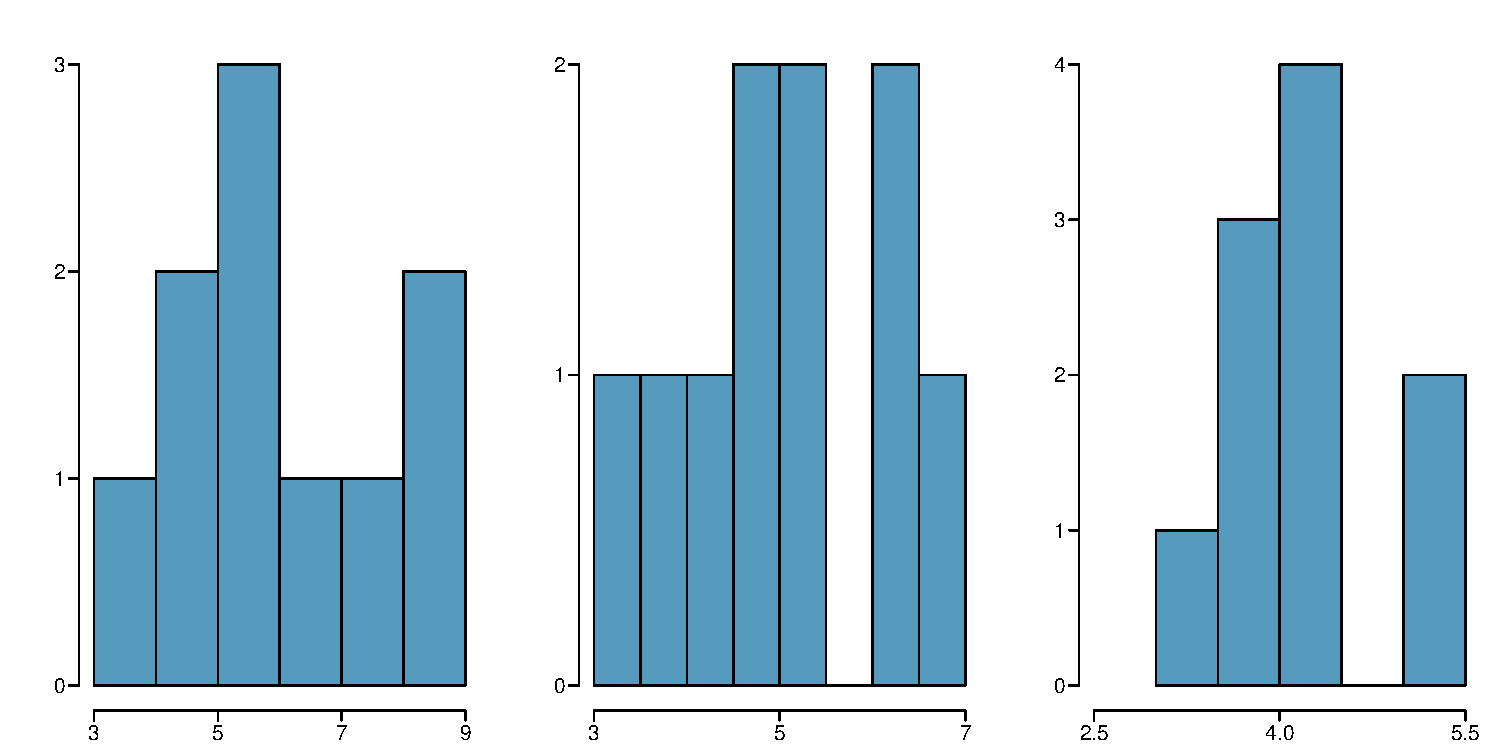
\includegraphics[width=\textwidth]{7-5_anova/figures/aldrin/normal}
\end{center}

\end{frame}

%%%%%%%%%%%%%%%%%%%%%%%%%%%%%%%%%%%

\begin{frame}[fragile]
\frametitle{（3）等分散性}

\dq{この条件は満たされているように見えるか？}

\begin{center}
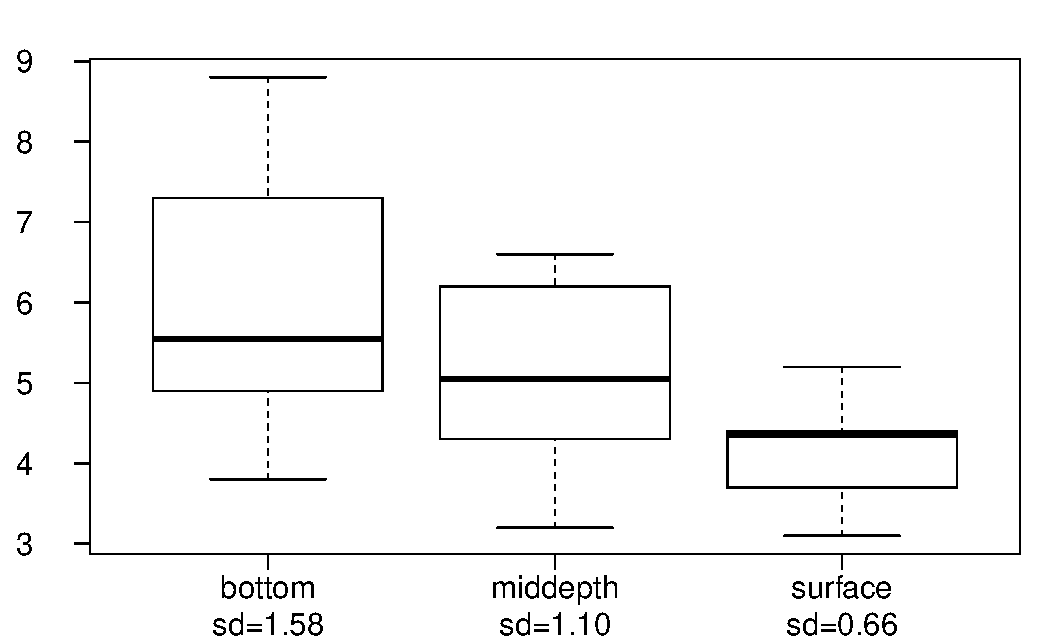
\includegraphics[width=0.7\textwidth]{7-5_anova/figures/aldrin/homo}
\end{center}

\end{frame}

%%%%%%%%%%%%%%%%%%%%%%%%%%%%%%%%%%%

\subsection{多重比較と第一種の過誤率}

%%%%%%%%%%%%%%%%%%%%%%%%%%%%%%%%%%%

\begin{frame}
\frametitle{どの平均が異なるか？}

\begin{itemize}

\item 先ほど少なくとも1対の平均が異なると結論付けた。自然に続く問いは「どの平均が？」である。

\item グループの全ての可能なペアについて2標本$t$検定を行うことができる。

\end{itemize}

\dq{このアプローチに潜在的な問題点は見えるか？}

\begin{itemize}

\item 多くの検定を行うと、第一種の過誤率が増加する。

\item この問題は修正された有意水準を使用することで解決される。

\end{itemize}

\end{frame}

%%%%%%%%%%%%%%%%%%%%%%%%%%%%%%%%%%%

\begin{frame}
\frametitle{多重比較}

\begin{itemize}

\item 多くのペアのグループを検定するこのシナリオを\hl{多重比較}（対比較）と呼ぶ。

\item \hl{ボンフェローニ補正}は、これらの検定にはより\orange{厳格な}有意水準が適切であることを示唆する：

\[ \alpha^\star = \alpha / K \]

ここで$K$は検討している比較の数である。

\item $k$グループがある場合、通常すべての可能なペアが比較され、$K = \frac{k (k - 1)}{2}$となる。

\end{itemize}

\end{frame}

%%%%%%%%%%%%%%%%%%%%%%%%%%%%%%%%%%%

\begin{frame}
\frametitle{修正$\alpha$の決定}

\pq{アルドリンデータセットでは深さに3つのレベル（底部、中深度、表面）がある。$\alpha = 0.05$の場合、どのペアの平均に有意差があるかを判断する2標本$t$検定の修正有意水準はどれであるべきか？}

\begin{enumerate}[(a)]
\item $\alpha^* = 0.05$
\item $\alpha^* = 0.05 / 2 = 0.025$
\solnMult{$\alpha^* = 0.05 / 3 = 0.0167$}
\item $\alpha^* = 0.05 / 6 = 0.0083$
\end{enumerate}

\end{frame}

%%%%%%%%%%%%%%%%%%%%%%%%%%%%%%%%%%%

\begin{frame}
\frametitle{どの平均が異なるか？}

\pq{以下の箱ひげ図に基づいて、どの平均が有意に異なると予想されるか？}

\twocol{0.6}{0.4}{
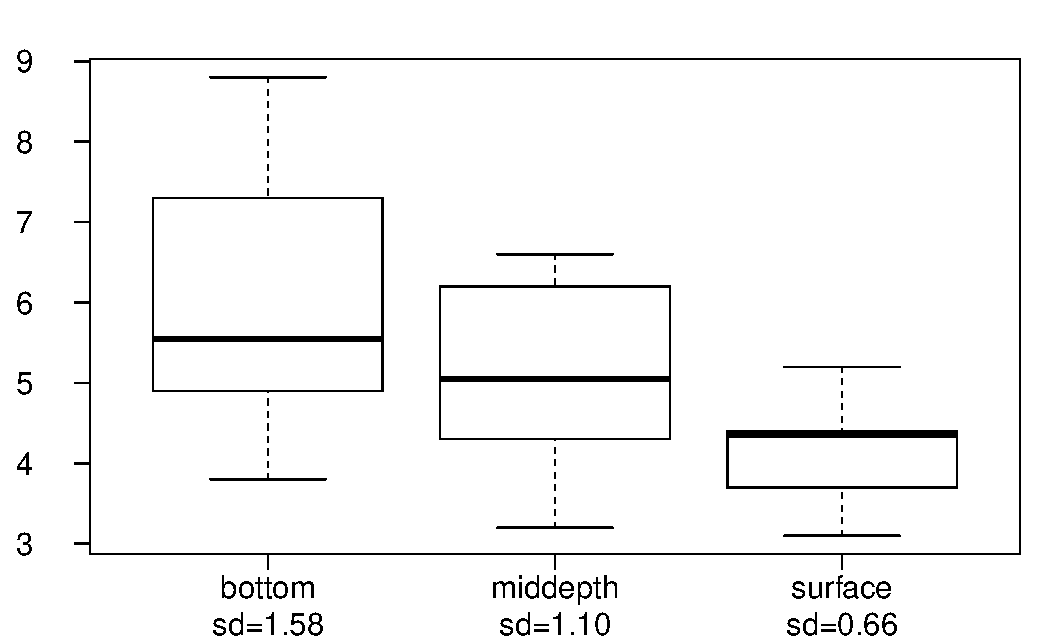
\includegraphics[width=\textwidth]{7-5_anova/figures/aldrin/homo}
}
{
\begin{enumerate}[(a)]
\item 底部 \& 表面
\item 底部 \& 中深度
\item 中深度 \& 表面
\item 底部 \& 中深度；中深度 \& 表面
\item 底部 \& 中深度；底部 \& 表面；中深度 \& 表面
\end{enumerate}
}

\end{frame}

%%%%%%%%%%%%%%%%%%%%%%%%%%%%%%%%%%

\begin{frame}
\frametitle{どの平均が異なるか？（続き）}

ANOVAのグループ間で等分散性の仮定が満たされる場合、すべてのグループのデータを使って変動性を推定できる：

\begin{itemize}

\item グループ内の標準偏差を$\sqrt{MSE}$（これが$s_{pooled}$）で推定する

\item $t$分布には誤差の自由度$n - k$を使う

\end{itemize}

\formula{2つの平均の差：ANOVA後}{
\[ SE = \sqrt{  \frac{\sigma_1^2}{n_1} + \frac{\sigma_2^2}{n_2} } \approx \sqrt{ \frac{MSE}{n_1} + \frac{MSE}{n_2} } \]
}

\end{frame}

%%%%%%%%%%%%%%%%%%%%%%%%%%%%%%%%%%

\begin{frame}[shrink=10]
\frametitle{}

\dq{底部と中深度での平均アルドリン濃度に差があるか？}

\twocol{0.4}{0.7}{
{\scriptsize
\begin{center}
\begin{tabular}{l | c c c}
		& n	& 平均	& 標準偏差	\\
\hline
底部	& 10	& \orange{6.04}	& 1.58 \\
中深度	& 10	& \orange{5.05}	& 1.10 \\
表面	& 10	& 4.2 	& 0.66 \\
\hline
全体	& 30	& 5.1		& 1.37
\end{tabular}
\end{center}
}
}
{
{\scriptsize
\begin{center}
\begin{tabular}{l rrrrr}
\hline
 			& Df 	& Sum Sq	& Mean Sq 	& F value 	& Pr($>$F) \\
\hline
depth 		& 2 	& 16.96 	& 8.48 		& 6.13 	& 0.0063 \\
Residuals 	& \orange{27} 	& 37.33 	& \orange{1.38} 		&  		&  \\
\hline
Total			& 29	& 54.29 \\
\end{tabular}
\end{center}
}
}

{\footnotesize
\begin{eqnarray*}
T_{df_E} &=& \frac{(\bar{x}_{\text{底部}} - \bar{x}_{\text{中深度}})}{\sqrt{ \tfrac{MSE}{n_{\text{底部}}} + \tfrac{MSE}{n_{\text{中深度}}} }} \\
T_{27} &=& \frac{( 6.04 - 5.05 )}{\sqrt{ \tfrac{1.38}{10} + \tfrac{1.38}{10} }} = \frac{0.99}{0.53}  =1.87 \\
0.05 &<& p\text{値} < 0.10 \quad \text{（両側）} \\
\alpha^\star &=& 0.05 / 3 = 0.0167
\end{eqnarray*}
}

{\small $H_0$を棄却しない。データは底部と中深度での平均アルドリン濃度に差がある説得力ある証拠を提供していない。}

\end{frame}

%%%%%%%%%%%%%%%%%%%%%%%%%%%%%%%%%%

\begin{frame}
\frametitle{}

\app{対比較}{底部と表面での平均アルドリン濃度に差があるか？}

\soln{
{\footnotesize
\begin{eqnarray*}
T_{df_E} &=& \frac{(\bar{x}_{\text{底部}} - \bar{x}_{\text{表面}})}{\sqrt{ \tfrac{MSE}{n_{\text{底部}}} + \tfrac{MSE}{n_{\text{表面}}} }} \\
T_{27} &=& \frac{( 6.04 - 4.2 )}{\sqrt{ \tfrac{1.38}{10} + \tfrac{1.38}{10} }} = \frac{1.84}{0.53}  =3.47 \\
p\text{値} = 0.0018 \qquad \text{（両側）} \\
\alpha^\star &=& 0.05 / 3 = 0.0167
\end{eqnarray*}
}
{\small $H_0$を棄却する。データは底部と表面での平均アルドリン濃度に差がある説得力ある証拠を提供している。}
}

\end{frame}

%%%%%%%%%%%%%%%%%%%%%%%%%%%%%%%%%%
